\documentclass[11pt,a4paper]{article}
\usepackage[utf8]{inputenc}
\usepackage[german]{babel}
\usepackage{amsmath}
\usepackage{amsfonts}
\usepackage{subfig}
\usepackage{amssymb}
\usepackage{siunitx,physics}
\usepackage{mathtools}
\usepackage{graphicx}
%\usepackage{Here}
\usepackage[version=4]{mhchem}
\usepackage{url}
\usepackage{setspace}
\usepackage[left=2.5cm,right=2.5cm,top=2.5cm,bottom=2cm]{geometry}
[biblography=totocnumbered]
\usepackage{fancyhdr}
\usepackage{scrextend}
\usepackage{hyperref}
\pagenumbering{gobble}

\makeatletter
\newcommand\bigcdot{\mathpalette\bigcdot@{.5}}
\newcommand\bigcdot@[2]{\mathbin{\vcenter{\hbox{\scalebox{#2}{$\m@th#1\bullet$}}}}}
\makeatother

\makeatletter
%\renewcommand*\bib@heading{%
%  \subsection*{}%
%  \@mkboth{\refname}{\refname}}
%\makeatother
\numberwithin{equation}{section}
\numberwithin{figure}{section}

\renewcommand{\labelitemii}{\labelitemfont$\vartriangleright$}
\begin{document}\\
\begin{addmargin}[25pt]{0pt}
\begin{figure}[h]
    \centering
    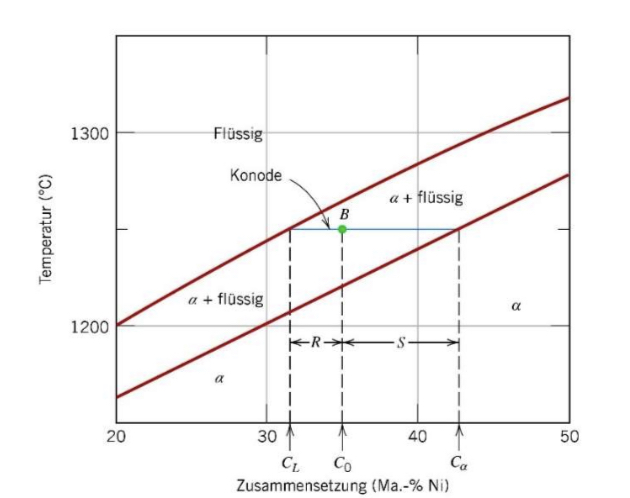
\includegraphics[width = 0.8\textwidth]{images/Materialwissenschaften/Zweiphasengebiet_Konode.jpeg}
    \caption{Das Zweiphasengebiet mit den Konoden $R$ und $S$ zur Bestimmung der Zusammensetzung von Schmelze und Kristall bzw. zur Bestimmung der Mengenanteile der Phasen.}
    \label{fig:zweiphasengebiet_konode}
\end{figure}
In Abbildung \ref{fig:zweiphasengebiet_konode} ist ein Punkt B im Zwei-Phasen-Gebiet eines Phasendiagramms dargestellt. Um die Zusammensetzung der Phasen zu bestimmen nutzt man Konoden, das sind Isothermen im Zweiphasengebiet. Die Schnittpunkte dieser Konoden mit der Solidus- bzw. Liquiduslinie geben die Zusammensetzung der festen bzw. flüssigen Phase an. In diesem Beispiel enthält die feste Phase $C_\alpha \approx 42,5\%$  Nickel wohingegen die flüssige Phase nur $C_L \approx 31,5\%$ Nickel enthält.\\
\end{addmargin}

\end{document}